\chapter{Componenti del Progetto}\label{ch:chapter2}
In questo capitolo verranno mostrati gli strumenti utilizzati per la creazione del \textit{framework}, che riproduce l'apprendimento del \textit{Continual Learning}.
\section{PyTorch}
\textbf{PyTorch} è una libreria di \textit{Machine Learning} open source basata sulla libreria \textbf{Torch}, utilizzata per applicazioni come la visione artificiale e l'elaborazione del linguaggio naturale, sviluppata principalmente dal laboratorio di ricerca AI di Facebook. È un software gratuito e open source nato  per essere utilizzato con il linguaggio di Programmazione Python(come avviene in questo elaborato), ma presenta  anche un'interfaccia C ++.
È stata utilizzata questa libreria perchè fornisce due specifiche molto utili per lavorare con le Reti Neurali: \textit{Pytorch Tensor} e i Moduli (AutoGrad ,Optim, nn).
PyTorch definisce una classe chiamata \textit{Tensor} (torch.Tensor) per memorizzare e operare su array di numeri rettangolari multidimensionali omogenei.
\newpage
\subsection{PyTorch Tensor}
I tensori PyTorch sono simili agli array NumPy, ma possono essere utilizzati anche su una GPU Nvidia compatibile con CUDA. Per lavorare al \textbf{Visual Recognition} è molto utile l'utilizzo della GPU: i tempi e le perfomance ne risentono in positivo.
\subsection{Moduli}
PyTorch utilizza un metodo chiamato \textit{automatic differentiation} (\textbf{AutoGrad Module}). Un \textit{Recorder} registra le operazioni eseguite, quindi le riproduce all'indietro per calcolare i gradienti. Questo metodo è particolarmente potente quando si costruiscono reti neurali per risparmiare tempo in un'epoca calcolando la differenziazione dei parametri nel passo del \textit{Forward}.
\newline
Il secondo Modulo che ci interessa è \textbf{Optim Module}(\textit{torch.optim}).
È un modulo che implementa vari algoritmi di ottimizzazione utilizzati per la creazione di reti neurali. La maggior parte dei metodi più usati sono già supportati, quindi non è necessario crearli da zero. In particolare l'algoritmo di \textit{ottimizzazione} che è stato scelto in questo elaborato è \textit{optim.SGD}, il quale implementa lo \textit{stochastic gradient descent}.
Durante il \textit{training} si adotteranno i metodi della classe \textit{optim} come \textit{ .zero\_grad()} e successivamente \textit{.step()} per fare l'update dei parametri della rete.
\newline
Infine abbiamo il modulo \textbf{\textit{torch.nn}} che ci fornisce molte più classi  per implementare e addestrare la \textit{rete neurale}. In particolare ci aiuta nella definizione della \textit{rete neurale}, e in quella dei \textit{layers} che la formano.
\newpage
I \textit{Packages} utilizzati in questo elaborato sono:
\begin{itemize}
    \item \textit{torch.nn.Module}: è una classe base per tutti i moduli di \textit{Rete Neurale}
    \item \textit{torch.nn.Linear}: utilizzato per i  \textit{layer Fully Connected}
    \item \textit{torch.nn.Conv2d}: utilizzato per i \textit{Layer Convoluzionali}
    \item \textit{torch.nn.MaxPool2d}: utilizzato per applicare un max pooling 2D 
    \item \textit{torch.nn.ReLU}: funzione di attivazione dei \textit{layer}
    \item \textit{torch.nn.CrossEntropyLoss}: funzione per il calcolo della \textit{Loss} della rete
\end{itemize}
Tutte le nozioni su \textit{Pytorch} e sui suoi \textit{Module} e  sui \textit{Tensori} sono stati presi come riferimento i \textit{docs} di \textit{PyTorch} \cite{pytorch}, \cite{pytorch_datasets} e \cite{pytorch_optim}.
\section{Dataset} 
\subsection{CIFAR-10}
Il dataset utilizzato in questo elaborato è \textbf{CIFAR-10}.
Esso è costituito da 60000 immagini a colori (avranno 3 canali per ciascuna immagine per gestire l'RGB) 32x32 divise in 10 classi, con 6000 immagini per classe. Sono disponibili 50000 immagini di allenamento e 10000 immagini di prova, come viene descritto in \cite{Cifar}.\newline
Il dataset è suddiviso in cinque \textit{batches} di Training e un batch di \textit{testing}, ciascuno con 10000 immagini. Il \textit{batch} di prova contiene esattamente 1000 immagini selezionate casualmente da ciascuna classe. I \textit{batches} di \textit{training} contengono le immagini rimanenti in ordine casuale, ma alcuni di essi possono contenere più immagini di una classe rispetto a un'altra. In  particolare, i \textit{batches} di \textit{training} contengono esattamente 5000 immagini di ciascuna classe.
\newpage
In questa immagine possiamo notare le dieci \textbf{classi} di \textbf{CIFAR-10} oltre a dieci esempi presi in maniera casuale da ciascuna classe.
\begin{figure}[ht]
\centering
\caption{Classi di CIFAR-10}
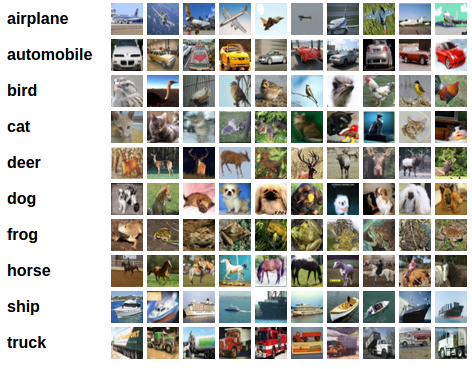
\includegraphics[width=\linewidth]{img/CIFAR.png}
\label{figure : CIFAR-10}
\end{figure}

\subsection{Gestione del Dataset}
Alla base della gestione dei \textbf{}{dataset} vi è la classe \textit{torch.utils.data.DataLoader}.
In particolare tutti  sono sottoclassi di torch.utils.data.Dataset, ovvero presentano  i metodi \textit{getitem()} e \textit{len()} implementati.
\newline
Per gestire il dataset \textbf{CIFAR-10} è stato istanziato nel progetto una classe \textit{Filtered\_dataset} che si occupasse di questa mansione.
L'obbiettivo dell'elaborato era rappresentare il problema del \textbf{Continual Learning} e per fare ciò è stato necessario dividere il dataset utilizzato in \textbf{\textit{tasks}}.
Ciò significa che a seconda del numero di \textit{tasks} che si vuole utilizzare per simulare il \textbf{Continual Learning}
sarà diviso il dataset per \textit{labels}. Ad esempio se si volesse utilizzare 5 \textit{tasks},  ognuno di essi conterrebbe 2 \textit{labels}.\newline
La classe \textit{Filtered\_dataset} si occupa di creare dei \textbf{subsets} con con il metodo della libreria di \textbf{PyTorch} \textit{torch.utils.data.Subset} che crea quest'ultimi dal dataset originario, supportato dal metodo \textit{idx\_tasks} (usato per la divisione delle \textit{Labels} nei \textit{tasks}).
Nel processo di suddivisione del dataset è stato necessario \textit{"mappare"} le \textit{labels} del dataset in modo tale da essere coerenti con l'output della rete. In particolare ciò è stato fatto tramite due attributi della classe \textit{Filtered\_dataset}:\textit{original2task} e \textit{task2original}. Questi due attributi consistono in due dizionari con chiave-valore, le \textit{labels} e la rispettiva mappatura.
Si reso inoltre possibile \textit{randomizzare} le \textit{labels} all'interno di ciascun \textit{task} per poter fare ulteriori \textit{tests} con il metodo \textit{idx\_tasks}.
\newline
\section{Rete Neurale Convoluzionale}
La \textbf{Rete Neurale Convoluzionale} (CNN o ConvNet) è una classe di \textit{reti neurali} profonde, molto spesso  applicata all'analisi ed al riconoscimento delle immagini.
La \textbf{Rete Neurale Convoluzionale} utilizzata in questo progetto è formata da sei \textit{Conv2D} layers separati da due \textit{MaxPool2D} ed infine da due \textit{Fully Connected Layer} sui cui ho applicato \textit{Dropout} per limitare l'\textit{overfitting} durante il \textit{training}. Per la scelta della conformazione della rete e per le definizioni delle tipologie dei vari \textit{layers} ho seguito il libro \cite{DeepLearningPython} e i docs di \textit{PyTorch}.
La particolarità di questa rete è che il \textit{layer} dell'output è \textbf{\textit{Dinamico}}, cioè che cambia a seconda del numero di \textit{tasks} su cui si vuole lavorare e sulla tipologia di approccio scelto tra \textit{Task-Agnostic} e \textit{Task-Aware}.
In particolare è possibile aggiungere nuovi \textit{layers} di output con il metodo\textit{add\_task} che richiama semplicemente il metodo \textit{add\_module} della classe \textit{nn.Module}.
Un altro metodo importante della \textit{rete neurale} sarà  \textit{set\_tasks} che  permette di settare il numero di \textit{tasks} voluti come output. I due attributi fondamentali della classe \textit{net} sono \textit{task\_fcs} e \textit{current\_tasks}, che sono sostanzialmente due \textit{array} contenenti gli indici dei \textit{tasks}. Il primo conterrà tutti i \textit{layers} lineari per le varie  \textit{Classification Head}, mentre il secondo, seleziona quale(i) task(s) sono correntemente attivi.
Qui di seguito si illustra la \textit{rete neurale} per un singolo \textit{task} con tutte le classi corrispondenti al \textit{Joint Training}:
Net(\\
  (conv1): Conv2d(3, 32, kernel_size=(3, 3), stride=(1, 1), padding=(1, 1))\\
  (conv2): Conv2d(32, 64, kernel_size=(3, 3), stride=(1, 1), padding=(1, 1))\\
  (conv3): Conv2d(64, 64, kernel_size=(3, 3), stride=(1, 1), padding=(1, 1))\\
  (pool): MaxPool2d(kernel_size=2, stride=2, padding=0, dilation=1, ceil_mode=False)\\
  (conv4): Conv2d(64, 128, kernel_size=(3, 3), stride=(1, 1), padding=(1, 1))\\
  (conv5): Conv2d(128, 128, kernel_size=(3, 3), stride=(1, 1), padding=(1, 1))\\
  (conv6): Conv2d(128, 256, kernel_size=(3, 3), stride=(1, 1), padding=(1, 1))\\
  (fc1): Linear(in_features=16384, out_features=120, bias=True)\\
  (fc2): Linear(in_features=120, out_features=84, bias=True)\\
  (dropout): Dropout(p=0.5, inplace=False)\\
  (task0\_fc): Linear(in_features=84, out_features=10, bias=True) )

\newpage
Il \textit{layer} \textit{Task0\_fc} è l'ultimo che è stato aggiunto con \textit{add\_task} e \textit{settato} con \textit{set\_task}.
Se l'esperimento fosse stato condotto su più \textit{tasks} ci sarebbero stati altri \textit{layers} oltre a \textit{Task0\_fc}. Nel caso in cui l'output voluto fosse stato su più tasks, nel metodo \textit{Forward} della rete tramite \textit{torch.cat}, sarebbero stati concatenati tra di loro i parametri corrispondenti selezionati da \textit{current\_tasks}.
\newline
La \textit{Funzione di Attivazione} utilizzata nei  \textit{layers convoluzionali} è \textbf{ReLu}, come anticipato precedentemente.
La \textbf{rectified linear activation function} o \textbf{ReLU} in breve è una funzione lineare a tratti che darà  come output direttamente l'input se è positivo, altrimenti produrrà zero. L'utilizzo della \textbf{ReLu} consente di ottenere un \textit{training} e una performance migliori.
\newline
Per quanto riguarda la funzione che si occupa del calcolo della \textit{Loss} è stata selezionata la \textbf{CrossEntropyLoss}. Questa funzione combina in una unica classe \textit{nn.LogSoftmax()} e \textit{ nn.NLLLoss()}.
Come anticipato nel paragrafo relativo a \textbf{PyTorch} è stato utilizzato come \textit{optimizer} \textbf{SGD} con \textit{Learning Rate} pari a  \mathbf{0.001}.\newline
Infine, è stato reputato necessario applicare \textbf{Dropout} ai due \textit{Fully Connected Layer} che precedono il \textit{layer} di output dinamico. Durante il \textit{training} azzera in modo casuale alcuni degli elementi del tensore di input con probabilità \textit{p} utilizzando campioni da una distribuzione di Bernoulli. In questo modo è stata ottenuta una diminuzione dell'\textit{overfitting}  riscontrato nella \textit{rete}.